\section{Knowledge Management System}
\label{sec:kms}

We first need to define what is the basic underlying system we build.
How knowledge is compared with data, information, and wisdom.
Then what is knowledge, \ac{KM}, \ac{KMS}, and micro \ac{KMS}.

% --------------------------------------------------
\subsection{Data-Information-Knowledge-Wisdom}

Between data, information, knowledge, wisdom; each of them has their interconnection with each other. Simply put:

\begin{dinglist}{220}
\item Data is the set of facts that already measured
\item Information is the processed data that could be useful (the what, when, where, who)
\item Knowledge is the contextual application of data and information (the how)
\item Wisdom is the evaluated understanding and appreciation of knowledge (the why)
\end{dinglist}

We can even define vision, a future predicted knowledge which is evolved from wisdom.
Figure \ref{fig:kms:dikw-pyramid} illustrates their connection hierarchy as a pyramid structure.

\begin{figure}[htbp]
    \centering
    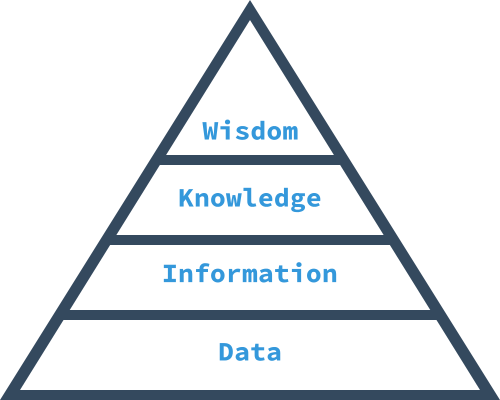
\includegraphics[width=4cm]{\dir/include/dikw-pyramid.png}
    \caption[DIKW Pyramid]{DIKW pyramid illustration about its hierarchy}
    \label{fig:kms:dikw-pyramid}
\end{figure}

% --------------------------------------------------
\subsection{Knowledge}

Generally defined, knowledge is facts, information, and skills acquired by a person through experience or education.
Processed information that bring out insights and undestandings, even processes that can be practiced.
It is the theoretical or practical understanding of a subject, known in a particular field or in total.
Others defined it as an awareness or familiarity gained by experience of a fact or situation.
In general, it is which we are understanding that germinates from combination of data, information, experience, and individual interpretation.~\autocite{BD2015Knowledge}

% --------------------------------------------------
\subsection{Knowledge Management}

\ac{KM}\index{knowledge management} could be defined as the process of applying a systematic approach to the capture, structure, management, and dissemination of knowledge throughout an organization in order to work faster, reuse best practices, and reduce costly rework from project to project.~\autocite{Dalkir2005KM}
\ac{KM} itself has already been created before its term exist, since the era of industrialization (circa 1800) and mostly used for corporate necessities.
Hence, \ac{KM} can be performed without the help of a computer, with just manual operation by human.

\begin{figure}[htbp]
    \centering
    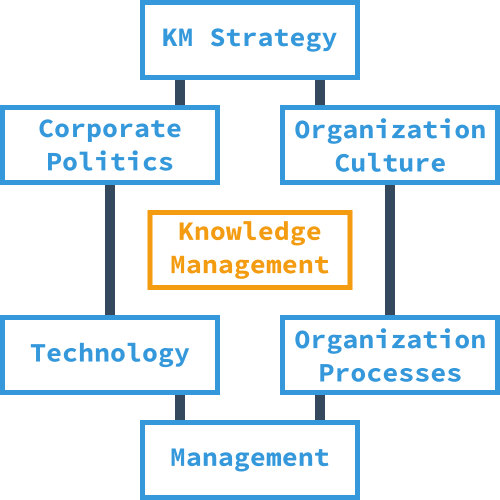
\includegraphics[width=5cm]{\dir/include/km-dimensions}
    \caption{Knowledge Management Dimensions}
    \label{fig:kms:dimensions}
\end{figure}

As knowledge management is essentially about getting the right knowledge to the right person at the right time~\autocite{Frost2010KM}, there are various factors around \ac{KM} that must be noted like in \autoref{fig:kms:dimensions}:

\begin{description}
  \item [KM Strategy]: The objective to take care of knowledge assets
  \item [Organizational Culture]: The influence of people interaction
  \item [Organizational Processes]: The implementation enabler
  \item [Management \& Leadership]: The competent and experienced team
  \item [Technology]: The systems, tools, and technologies that fit the requirements
  \item [Politics]: The long-term support to implement and sustain initiatives
\end{description}

% --------------------------------------------------
\subsection{Knowledge Management System}

\ac{KMS}\index{knowledge management system} that also can be called knowledge manager, is a method for the improvement of business process performance.
It is most often used in business in applications such as information systems, business administration, computer science, public policy, and general management.
Common company departments for knowledge management systems include human resources, business strategy, and information technology.~\autocite{BD2015KMS}
In short, \ac{KMS}s are tools aimed at supporting knowledge management.~\autocite{Dalkir2005KM}
Nowadays \ac{KMS} can be handled with a great deal of computer system, network, and people together.

In this context, it is more and beyond that, because \ac{KMS} can:

\begin{easylist}
& Comprises a range of practices used in an organization to identify, create represent distribute and enable adoption to insight and experience
& Be such insights and experience comprise knowledge, either embodied in individual or embedded in organizational processes and practices.
\end{easylist}

So it is the thing of storing and managing these kinds of knowledge in a decent friendly ecosystem that has:

\begin{easylist}
& Personalized information
& State of knowing and understanding
& Object to be stored and manipulated
& Process of applying expertise
& Condition of access to information
& Potential to influence action
\end{easylist}

Related to our solution, if Satellid is compared against its most similar or popular tools in terms of storing data, information, and knowledge, \autoref{table:kms-comparison} can summarize the difference. Note that not every tools mentioned are genuinely made to be a knowledge manager, but users could decide them inderectly from an encyclopedia, note taking app, or data platform, to be a knowledge manager.

\begin{table}[h!]
\centering
\begin{tabular}{ |c||c|c|c|c|c| }
\hline
Type         & Satellid   & Evernote      & Google Keep & Wikipedia    & Silk \\ \hline
\hline
Focus        & Knowledge  & Notes         & Notes       & Encyclopedia & Data \\ \hline
\shortstack{Data\\Format} & JSON       & ENML          & JSON        & XML/Wiki     & JSON \\ \hline
Vision       & Ubiquitous & \shortstack{Business\\Work} & Casual Use  & \shortstack{Public,\\Academic} & Visualization \\
\hline
\end{tabular}
\caption{KMS-related tools comparison}
\label{table:kms-comparison}
\end{table}

The type defines characteristic of each tools: focus is the primary substance usage of it, data format is the primary system to store and exchange data inside or outside the software, and vision is both the initial and real use case.
As an important note, the initial version of Satellid may not be complete as the others currently have.
For now we still only processes text data as the main features.

% --------------------------------------------------
\subsection{Micro {KMS}}

It is simply defined as the simplified and minimized version of \ac{KMS}.
The micro approach allow us to start the system as small as possible but can be enlarged and adapted into any size.
Unlike any other concept and implementation of commonly defined as micro knowledge management system, this procedure takes on the essence of the system scale.
In a simple matter, micro \ac{KMS} has a very small size as in both file, system, and architecture size.

% --------------------------------------------------
\subsection{Knowledge Base}

Explaining a bit about \ac{KB}\index{knowledge base} and how it is different from \ac{KMS} can be likened as comparing encyclopedia and comprehensive library with various type of contents.
\ac{KB} is like encyclopedia, mostly storing just collection of information without concerning much about process and meaning.
But \ac{KMS} is like comprehensive library, more into collection of knowledge that can be used with and processed for specific context, because there are plenteous of them ranging from stories to catalogues to tutorials.
Also, \ac{KB} is closely related to database while \ac{KMS} can even be done without a database but just collections of knowledge in various formats and sources.
\ac{KB} is likewise related to expert system, a system which depends on \ac{KB} for its substantial informations.
%In conclusion, \ac{KB} encompasses the technology for storing all kinds of information that oftentimes using computer system.
